\begin{figure}
  \centering
  \subfloat[]{%
    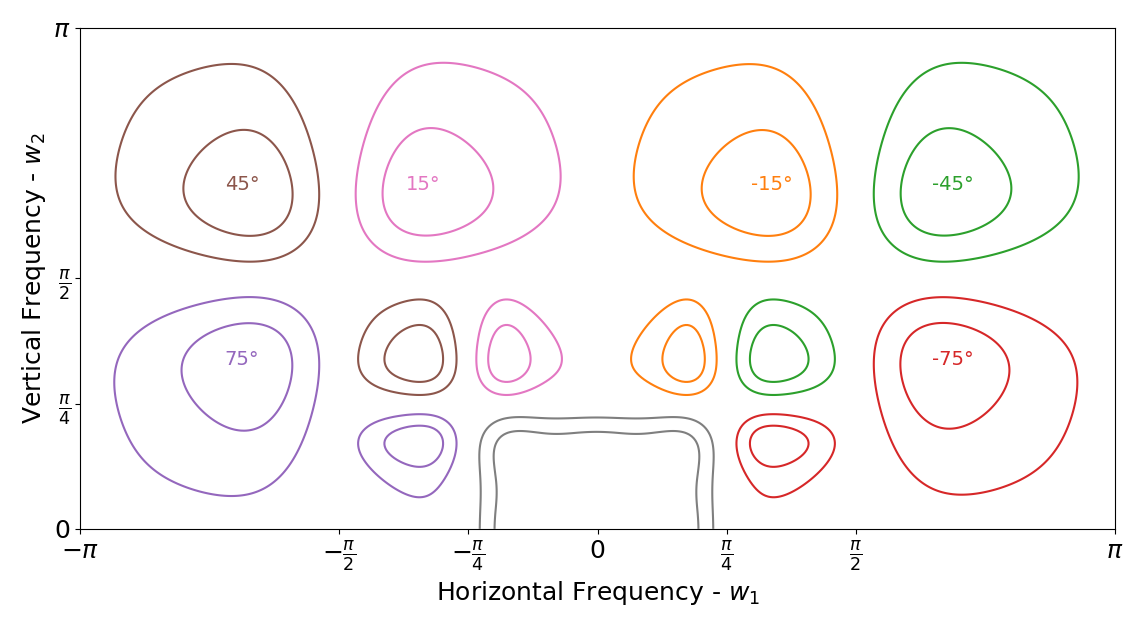
\includegraphics[height=6cm]{freqlearn/images/subbands.png}
    \label{fig:ch6:dtcwt_bands_freq}
  }
  \hspace{1cm}
%    \newline
  \subfloat[]{%
    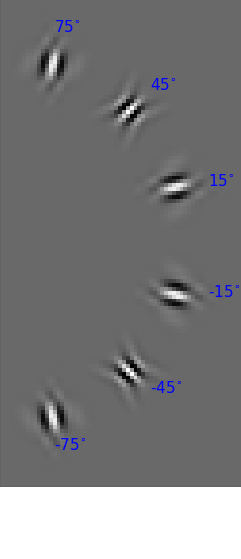
\includegraphics[height=5.7cm]{freqlearn/images/impulses.png}
    \label{fig:ch6:dtcwt_bands_impulse}
  }
  \newline
  \subfloat[]{%
    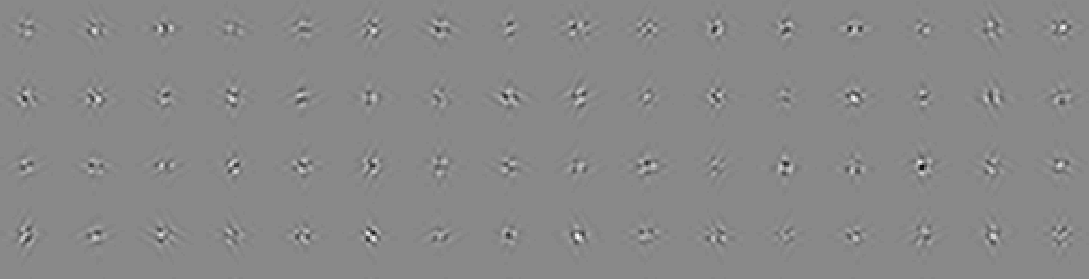
\includegraphics[width=\textwidth]{freqlearn/images/examples_scale2.png}
    \label{fig:ch6:example_impulses}
  }
  \mycaption{Frequency and Spatial support proposed gain layer}{\subref{fig:ch6:dtcwt_bands_freq} Contour plots at
    -1dB and -3dB showing the support in the Fourier domain of the 6 subbands of
    the $\DTCWT$ at scales 1 and 2, and the scale 2 lowpass. These are the 
    product $P(z)Q(z)$ from \autoref{eq:ch6:end_to_end1}.%
    \subref{fig:ch6:dtcwt_bands_impulse} The pixel domain impulse responses for
    the second scale wavelets. \subref{fig:ch6:example_impulses} Example
    impulses of our layer when $g_1$, and $g_{lp}$ are 0 and 
    $g_2 \in \mathbb{C}^{6\x 1\x 1}$, with each real and imaginary element 
    drawn from $\mathcal{N}(0,1)$. I.e., only information in the 6 subbands with 
    $\frac{\pi}{4} < |w_1|, |w_2| < \frac{\pi}{2}$ from 
    \subref{fig:ch6:dtcwt_bands_freq} is passed through.} 
  \label{fig:ch6:dtcwt_bands}
\end{figure}

